% Use the uit-report.cls to style the document
\documentclass{uit-report}



%%%% PREAMBLE ---- here you can add packages if you need extra functionality %%%%

% Provides the \lipsum command to create "Lorem Ipsum" sample text.
\usepackage{lipsum}
\usepackage{listings,multicol}
\usepackage{varwidth} %for the varwidth minipage environment
\usepackage{pdfpages}

\setcounter{tocdepth}{1}


\usepackage{enumitem}



\begin{document}
\title{Saddlebags: An Object-Oriented Parallel Computing Framework for C++}
\author{Aril Bernhard Ovesen}
\date{June 1, 2018}


% Saddlebags - A High Performance Computing Framework
%An object-oriented general-purpose parallel framework with UPC++

% Saddlebags - A distributed programming framework
% Achieving efficiency and expressiveness in data-intense and compute-intense applications with UPC++

\pagestyle{firststyle}
\setcounter{page}{1}
\section*{Abstract}
\addcontentsline{toc}{chapter}{Abstract}
The volume of data generated by web services and scientific tools is increasing more rapidly than many currently available high performance computing tools are able to keep up with. There is a need for novel data abstractions and parallel computing frameworks that can handle workloads from the fields of both high performance computing and big data analysis. This thesis presents Saddlebags, a high performance computing framework built on UPC++. Saddlebags aims to achieve high performance by coupling data and computing task together to exploit data locality. Principles such as fine grained remote data access and explicit data movement are inspired by high performance computing systems, while concepts such as implicit data distribution and fault tolerance are inspired by big data systems. Saddlebags can be used on individual nodes and on compute clusters, and achieves favorable performance when compared to other modern systems on both platforms.

\section{Introduction}


%  State of high performance computing
%  Shared memory and message passing
%  Role of different programming models/abstractions
%  Data centric computation
%  UPC++

%Scientific applications and engineering research are undergoing a transformation
%At the end of Dennard Scaling around 2004, transistor clock frequencies could not be raised without increasing the total circuit power consumption.
%Introduced multicore, manycore and accelerator-based computing 
%The big data revolution 
%Analysis, management, and collection of large volumes of data makes up the field of data-intensive science. 

%The core of high performance computing is writing efficient and parallel applications, which is the concern of researchers from an increasing range of disciplines, from physics and chemistry to medicine and geology. While the available hardware is being steadily improved,  \cite{engineering}. 


High Performance Computing (HPC) is becoming of increased importance for scientists and researchers of a large range of disciplines, from physics and chemistry, to medicine and geology. At the very core of HPC lies the ability to write efficient and parallel software~\cite{engineering}.

The U.S Department of Energy reported in 2013 through the Advanced Scientific Computing Advisory Subcommittee that the data volumes produced by scientific experiments and simulations were increasing more rapidly than the currently available algorithms, computing systems and workflows were able to keep up with. They also reported a need for innovations in HPC and data-intensive science to address challenges with contemporary systems related to concurrency, data movement, and energy efficiency~\cite{subcommittee}.

Big data frameworks such as Apache Hadoop~\cite{hadoop}, Spark~\cite{spark} and Flink~\cite{flink} can provide simple programming interfaces for distributed algorithms, with the underlying assumption that distribution of data and computing tasks can be handled by the system without programmer input. Programmers are given functionality to access data without explicitly managing communication between nodes. These systems are often reliant on coarse grained operations, which in many cases can produce inefficient programs, and limit the programmability of a framework~\cite{husky, piccolo}. Many data analytics operations are often orders of magnitude slower when implemented in a data analytics framework like Spark, than when written with native HPC tools such as MPI~\cite{bridgingthegap}. However, with a simple programming model, support for numerous data formats, underlying fault tolerance and automated data distribution, Spark remains an attractive option for distributed big data workloads~\cite{sparkarticle}. 

As many scientific applications depend on processing high volumes of data, problems of HPC and big data analytics are converging. As the amounts of data increase, so does the importance of developing more efficient analytical tools~\cite{hpcabds}. Features from big data systems can be incorporated into HPC frameworks, to create programming models that are intuitive and higher-level, yet expressive and performant. This thesis presents Saddlebags, a framework that attempts to strike a balance between the two paradigms of parallel computing systems. Inspired by big data frameworks, Saddlebags supports automatic distribution of data and computational tasks, and removes the need for specialized communication routines based on physical location. Inspired by HPC frameworks, Saddlebags allows fine grained memory access of distributed data, and leaves data movement during computations explicit and up to the programmer.

Saddlebags takes an approach to parallelism similar to graph frameworks \cite{pregel, giraph} that distribute data in vertices, and allow computational tasks to be executed within the context of each individual vertex. Saddlebags aims to support various classifications of workloads, including graph computation, and provides a vertex-like abstraction called Items. Applications are built with Saddlebags by extending an \texttt{Item} class, and creating custom item objects that contain data and computational tasks.

Saddlebags is implemented in C++. It uses parallelization and communication implementations from UPC++, a Partitioned Global Address Space library. With UPC++, a program has a static number of threads, each of which is given the affinity of a unique private memory segment. While data can be shared across segments, a memory segment is mainly accessed by the thread it has affinity to. Saddlebags applications can be used either on a single node or across multiple nodes within a compute cluster, using Ethernet or InfiniBand for network communication.



%while still allowing fine grained memory access, 


%Advantageous programming models from big data systems can be incorporated into 


%By incorporating concepts of simple programming models from big data systems, into HPC frameworks typically known for complex, we can develop tools that can solve problems that depend on both big data processing and performant computation.

%As the importance of advanced big data analytics

%Highly performant communication or computation a


%Designing efficient, yet intuitive programming models for distributed computing and data analytics seems to .

\section{Contributions}
In brief, we make the following contributions

\begin{itemize}
	\item We design and implement Saddlebags, a High Performance Computing framework and programming model that borrows features from several other HPC frameworks and big data systems, with the aim of supporting workloads of different classifications.
	\item With the implementation of this framework, we use the UPC++ PGAS library as a communication layer for more advanced abstractions. To our knowledge, this is the first HPC framework built with UPC++.
	\item We implement several different protocols for communication between concurrent partitions, and evaluate their performance characteristics.
\end{itemize}

\section{Related work} \label{section:relatedwork}
Several modern HPC frameworks and big data systems were used as a baseline for current starte of the art HPC techniques and programming models.

Pregel \cite{pregel} is a system for distributed graph processing, first presented in 2010. Pregel was designed to scalably process large graphs created by web services. The workflow of Pregel involves distributing the vertices of a graph across nodes in a cluster, and performing independent computational tasks on each vertex. These tasks are performed iteratively, meaning that individual vertices may execute tasks in parallel, but the beginning and end of an iteration is synchronous, equivalent to a Bulk Synchronous Parallel execution model. Pregel claims better performance than MapReduce-based workflows through passing messages directly to the nodes containing relevant vertices. This is in contrast to expressing a graph as a chain of application states, where the entire graph must be re-created and re-distributed for each iteration.

Apache Spark \cite{spark} is a framework for big data applications, initially released in 2014. Spark aims to provide a unified programming model for different distributed workloads that handles large amounts of data. Spark is based around Resilient Distributed Datasets (RDDs), an abstract data type that implicitly distributes data across nodes and provides fault tolerance through re-creation of the data on faulty nodes. RDD operations are coarse-grained and applies to the entire dataset per execution step. This means that operations applied to an RDD can easily be logged, and the entire dataset can be re-created in case of faults. Computations with RDDs can be represented as a directed acyclic graph (DAG), in which the RDD moves from one state to the next, by applying transformations on the entire data structure. RDDs are re-created by replaying the DAG.

Husky \cite{husky, husky_website} is a framework for HPC, large scale data mining and research of distributed algorithms. The programming model of Husky is based around two main concepts: firstly, distribution of programmer-defined objects that contain some data element, and secondly, programmer-defined computational tasks that can be executed on these objects. This distribution of data and tasks is similar to the Pregel definition of vertices. Objects can communicate with each other using a push-pull model, and functions executed on data can choose to parse through received pushes. The Husky paper shows experimental results in which Husky compares positively to other systems including Spark in several different workloads. With bulk data movement workloads, Husky explains superior performance through fine-grained data access. With graph analytics, Husky explains superior performance through optimized combination of communication messages, which reduces network bandwidth usage. 

\section{UPC++}
UPC++ is a PGAS extension to the C++ programming language. It is developed at University of California, Berkeley and saw the release of its 1.0 version in September 2017. UPC++ is implemented as a library extension, due to the complexity of developing a separate C++ compiler \cite{zheng_kamil_driscoll_shan_yelick_2014}. The library heavily utilizes C++ template programming \cite{web_cpp_template} for PGAS mechanisms, which allows the creation of library functions that use generic variables that can be adapted to different types. 

UPC++ follows the Single Program Multiple Data model and like UPC utilizes threads with affinity to memory partitions. While UPC++ allows the use of C++ functionality such as objects and lambdas, it still aims to provide high performance and explicit communication by leaving much responsibility regarding concurrency and data movement to the programmer.

Each UPC++ partition has access to its own private memory segment, and is identified by its \emph{rank}, an integer that can range from zero to the total number of partitions. Partitions of different ranks can communicate through a logical shared memory segment, by utilizing UPC++ communication functionality, including global pointers, Remote Procedure Calls (RPCs), and distributed objects. The number of ranks is static during execution; the total rank count is specified when launching a program and cannot be modified during runtime.

The 1.0 release of UPC++ introduced the concept of \emph{distributed objects}, which are objects defined by a generic type within UPC++ with the same identifier across all ranks. This means that data stored in the private memory segment of a partition can be referenced by a different rank in RPC calls. The data within the object is not implicitly distributed, but the name of the variable is. Local contents of the distributed objects can as such be explicitly distributed to any rank.

Outstanding asynchronous operations are not completed automatically, because the program consists of a static number of threads. In order to advance the internal state of UPC++ or complete RPC calls, computing resources are yielded from the main thread of execution via the \texttt{progress()} function. This concept puts the responsibility of frequently progressing UPC++ state on the programmer's shoulders. The goal of this is to provide visibility of resource usage and parallelism, the latter being important to achieve interoperability with libraries and software packages that would otherwise restrict the use of multi-threading. Being cautious about where to progress RPCs relieves the needs for concurrency control such as mutexes, and implies atomicity in partition-internal operations of basic data types. More complex data structures that are not designed for concurrent access can be safely referenced in RPCs across partitions as long as the \texttt{progress()} function is used only between atomic accesses.

\section{Design goals}
Some of the underlying concepts in Saddlebags and the motivation behind them follows:

\hspace{4ex} \textbf{1. Computational tasks should be expressed with a relationship to the data it requires, and executed in the same partition in which this data is located}

Problems that can be expressed with data parallelism can be distributed across computing units as individual tasks related to specific data. To exploit data locality, a computational task should only be performed on the unit of computing which the data it requires has affinity to. Computational tasks will have affinity to the data it requires, the same way data has affinity to a computing unit and its private memory segment. When a task requires multiple data items, communication with other partitions may be unavoidable.
\\

\hspace{4ex} \textbf{2. A multitude of data should be implicitly distributed across available partitions}

Following the principle of a computational task's affinity to its data, full utilization of available processing units is only possible when a program's data is distributed. This means that data used in parallel processing should always be distributed across available memory partitions, so that the computational tasks that require the data is equally distributed.
\\	

\hspace{4ex} \textbf{3. The programmer should not need to write communication routines such as messages or Remote Procedure Calls}

While computation methods are application-specific, communication patterns can be implemented for a general case. When claiming that programmers are relieved of writing communication routines, it refers to the need for knowing where data is physically stored, which partition to communicate with, and the need for ensuring that messages are delivered before continuing computation. Data movement will still be explicit, but expressed in an abstraction level in which data locality and memory partitioning is not considered. 
\\

The goal of building a a framework on these specific features is to allow computational parallelism to be expressed with the same semantics as data parallelism, while still allowing tasks to communicate data between each other. The complexity of implementing applications that fit this classification is reduced by utilizing a general communication pattern that relieves programmers of implementing specialized communication. Programmers will in this framework use communication routines by referring to data identifiers rather than physical location.

Like several of the systems mentioned in section \ref{section:relatedwork}, Saddlebags implements a Bulk Synchronous Parallel programming model. Like Pregel, Saddlebags distributes a generic and extendable computational task with every data item. Like Husky, Saddlebags provides a more flexible data movement model between items, and does not aim at supporting graph-oriented workloads exclusively.

\section{Programming model}
The programming model and data flow model of Saddlebags is based around coupling data and functionality together into an object. Objects that serve the purpose of executing computational tasks in Saddlebags are named \emph{Items}. Items contain pre-existing general communication methods, and the main effort of developing an application with Saddlebags is implementing the computational tasks within an item, and integrating communication and data-flow into that task.

Items of different types can be implemented in the same application, and stored in different tables. The behavior of these tables cannot be extended by the programmer, but every application must define their tables by name and item type. Tables are common for every partition, while an instance and name of an item can only exist on a single partition. This is how distribution of data is achieved: items are spread across partitions, while the tables that contain them exist on every partition, and can reference items regardless of physical location.

Items implement a \emph{work-push-pull} model, in which \emph{work} refers to a computational task implemented in the item class, and \emph{push} and \emph{pull} are the two available modes of communication. The work of an item is designed to be executed iteratively, and each iteration of a Saddlebags application involves executing work and performing any communication routines that was called as a result of the work. An iteration applies to every item in every table, and it is with this iterative model that an application can be executed. 

\subsection{Events} \label{section:events}
The data flow model of Saddlebags is implemented with the concept of \emph{events}. Within the context of this framework, an event refers to the receiving of any communication message, or reaching specific points of the iteration process. Whenever an event is triggered, for example when receiving a \emph{pull} message, the item that received an event-trigger calls a corresponding method, in this case a \emph{foreign pull} method. The contents of this method can be implemented differently in different item types, and is also able to initiate other communication routines. This is directly related to the data flow of an application: when receiving a pull event, the event-triggered method determines what data to return. When the message returns to the original sender with some data, the event-triggered return method determines how to handle the data. 

\begin{table}[h]
\setlength\arrayrulewidth{1pt}
\renewcommand{\arraystretch}{2}
\begin{tabular}{ | p{3cm} | p{6cm} | p{6cm} |}
   	\hline
   	\textbf{Method} & \textbf{Event} & \textbf{Implied data movement} \\ \hline
   	On Create & Item is created & None\\ \hline
  	Refresh & An item with the same name is attempted created & None \\ \hline
  	Work & Start of iteration & None \\ \hline
   	Foreign Push & A push message is received from another item & Data from sender is received with the message  \\ \hline
   	Foreign Pull & A pull message is received from another item & Return data is sent back to the sender\\ \hline
	Returning Pull & A pull message that originated in this item has returned & Data from pull target is received with the message\\ \hline
	Finishing Work & End of iteration & None\\ \hline

\end{tabular}
\caption{All events and their corresponding methods}
\label{table:events}
\end{table}

Table \ref{table:events} lists all methods in the item class that can be triggered by events. Column 1 lists the names of the methods, column 2 lists the circumstances under which the method is called, and column 3 lists what data is moved in the corresponding method.

All methods with data movement are called as a result of communication with other items. Communication routines can be initiated in any of the methods listed in the table. Items are referenced by name, so two items with the same name cannot exist in the same table. The \emph{Refresh} method is used to incorporate this behavior in a program.

\subsection{Data distribution}
Each table is initialized with a distributor type, a specific class with a distribution method that determines the partition in which items should be located. Since all data is stored in items, and all items are stored in tables, the distribution type of tables is the only component of a Saddlebags application that manages distribution of data and computation.

The distribution method that is common for all distributor classes takes an item name as parameter, and returns a partition identifier. By default, distribution is based on the hash digest of the item name, utilizing consistent hashing where items will be assumingly evenly spread around all partitions \cite{consistenthashing}. The motivation behind this is to distribute computational tasks as evenly as possible.

When a table is created, it is specified whether it is a local or global table. Global tables utilize distributors, that can potentially distribute data across all partitions that are available in the system. Local tables does not utilize any distribution logic, and all items are stored within the same partition as they were created. While local tables are created on every partition, their items cannot be remotely accessed. The items in global tables can always be remotely accessed, regardless of their distribution~model. From a programming standpoint, communication with local or global tables looks identical, but setting the locality of a table can have an impact from a data movement and optimization standpoint, since communication with a local table will never implicitly invoke remote operations.


%The communication patterns of a push/pull paradigm is simple enough that the cost of data movement as a result of communication in an application can be reasoned about, despite implementation complexity being hidden. 

%Saddlebags is designed with the goal that abstractions provided by the programming model, through C++ mechanisms such as inheritance and type templates, should not affect algorithmic complexity. This will likely only be true for algorithms that can be tailored to the push/pull/work paradigm. 

\section{Fault tolerance}
Saddlebags takes an approach to achieving a degree of fault tolerance by utilizing replication. Each partition will act as a replica for one or more partitions with subsequent rank values, looping back to partition 0 at the highest rank. The degree of fault tolerance, i.e. the number of replicas per partition, is defined on a per-application basis. This is similar to the hash ring approach found in the key/value storage system Dynamo \cite{dynamo} and the peer-to-peer hash table protocol Chord \cite{chord}.

Replicas are updated at the end of each iteration, which means that every node is in a state where no updates occur when replication routines are executed. This makes for low communication overhead during replication, since all contents of a table can be sent in one message. This raises an issue with inconsistency, if a node crashes during computation. A situation like this must be solved with a rollback operation, moving every table to the previous iteration. This is achievable with the same replication routines, since a back-up of the state of the previous iteration exists in the current replicas. This means that, to rely on rollbacks, a replication degree of at least 2 must be used. 

\section{Implementation}

The previous chapter presented an object-oriented approach to parallel computation, in which problems were split up into separate items that could be distributed and accessed independently of other items. Defining computational tasks in items, and passing data as messages between items with different tasks, is the main effort of implementing programs in Saddlebags. The final program structure of the framework was devised in the development of an interface in which items of different types were interoperable, through a common messaging interface.

Generic items are implemented as a C++ class, consisting of pre-defined communication methods, in addition to several empty methods, corresponding to the events listed in section \ref{section:events}. To develop meaningful programs, some of these events must be extended. This is done through inheritance. Event-methods are marked as \texttt{virtual}, so that they can be overridden. Non-event methods, such as push and pull, implement generic functionality that will remain the same for all item classes. This leaves the \texttt{virtual} methods to indicate the interface in which events can be implemented. 

Items are stored in hash maps, which are defined in a \texttt{TableContainer} class. The hash map and table container makes up the functionality of the table described in chapter~\ref{chapter:design}. \texttt{TableContainer} inherits from a \texttt{TableContainerBase} class that contains functionality that is applicable for all item types. The reason for this will be expanded on in section \ref{section:templates}. Table containers have default logic for distributing items across partitions, and this can be exchanged for specialized solutions by passing a \texttt{Distributor} object. The \texttt{Distributor} class implements a \texttt{Distribute()} method that takes a item key as parameter, and returns an integer corresponding to the rank in which that item should be stored. 

An application can consist of multiple tables, containing different item types. Tables are stored in the \texttt{Worker} class, which is responsible for synchronization, initiating computational tasks through the events \emph{Work} and \emph{Finishing work}, and providing a common interface for different items to access each other in order to deliver messages. Every table and item in a program can be referenced through its worker. A Saddlebags program is initiated by creating a worker, and there is little purpose in having multiple simultaneous workers.


\subsection{Sending modes} \label{section:sendingmodes}
Communication between items based on push and pull methods. Saddlebags implements several different techniques for handling these communication routines, which is determined by a \texttt{sending\_mode} property in the worker. The following modes are implemented.

\hspace{4ex} \textbf{\texttt{Buffering}}
\\
Push and pull operations are stored as messages, in which the table and item name of both the sender and receiver is stored. Messages are sent when the communication method is called, but received messages are buffered and not applied until after the work-phase is finished. The purpose of the buffering is to enforce a bulk synchronous parallel execution model.\\

\hspace{4ex} \textbf{\texttt{Combining}}
\\
Similar to the Buffering mode, but messages are not sent until the work-phase is completed, so that all messages with the same source and destination partitions are sent in a single RPC. This is implemented on the sender-side by buffering messages in an associative data structure with destination partition as key, and a vector of messages to that partition as value.\\

\hspace{4ex} \textbf{\texttt{Direct}}
\\
Operations are not stored intermediately as messages, but rather only expressed through the execution of its RPC. Does not enforce any synchronization, so push and pull operations can be executed both before or after work. \\

\hspace{4ex} \textbf{\texttt{GasnetBuffering}}
\\
Like the Direct mode, operations are only represented as an RPC. Like the Buffering mode, operations are performed in a bulk synchronous parallel pattern. This is achieved by not advancing UPC++ state, by not calling the \texttt{progress} function until all partitions has completed the work phase. This means that any buffering of operations is handled by the internal communication routines of GASNet. Other buffering techniques are preferred because GASNet cannot store more than 65536 outstanding operations \cite{gasnetpresentation}. This mode was implemented for the experimental purpose of removing the overhead of the Message abstraction.


% no synch for expansion etc due to progress
% one way communication futures are stored
% barriers in cycle
%
%\section{Usage}

\section{Evaluation}
Benchmarks were performed on three different systems:

The first system, a desktop machine, has an Intel Core i5-4460 CPU @ 3.20 GHz, with 4 cores and 256 KiB, 1 MiB and 6 MiB L1, L2, and L3 caches respectively. This system has 8 GB memory and runs Ubuntu 16.04.

The second system, a university provided server, has an Intel Xeon E5-2650L v3 CPU @ 1.80GHz, with 24 cores and 768 KiB, 3 MiB and 30MiB L1, L2, and L3 caches respectively. This system has 64 GiB memory and runs CentOS 7.5.1804.

The third system is the Abel computing cluster at the University of Oslo. Abel consists of 650+ compute nodes, with Intel E5-2670 CPUs @ 2.6 GHz, with 16 cores and 64 GiB memory. At this time, Abel uses CentOS 6 \cite{abel}. Nodes are connected with FDR InfiniBand. In this evaluation, only one core is used per node. This is the default behavior of the workload manager available on this cluster \cite{abeluserguide}, and the recommended way of running Spark jobs~\cite{abelspark}. 

This selection of systems is used because it allows for both single node and distributed workloads. The 4-core Ubuntu system is used because of compatibility issues with Husky and its dependencies and CentOS. The 24-core server is used so that single node benchmarks can be ran with more than 4 partitions.

PageRank and TF-IDF are used as benchmarks. PageRank benchmarks were performed on Kronecker graphs. Kronecker graphs are graphs modeled after properties from real networks, with the purpose of providing a scalable generative mathematical graph model \cite{leskovec2010kronecker}. For this evaluation, Kronecker graph generation was performed with the BigDataBench benchmark suite \cite{wang2014bigdatabench}.

\subsection{Comparison with Husky} \label{section:huskycomp}
A comparison with Husky was ran on the desktop system. A PageRank example program, from the official Husky repository was used. Husky was launched with 4 workers, which is equivalent to 4 parallel threads. Saddlebags was launched with 4 partitions, and uses the default sending mode, which is \texttt{Buffering}.

Results are shown in figure \ref{fig:huskypagerank}. In this benchmark, Saddlebags completed the task in shorter time than Husky on three different Kronecker graphs. It is shown that both the base execution time, and the scaling with dataset size, are slower in Husky than in Saddlebags.


\begin{figure}[H]
	\centering
	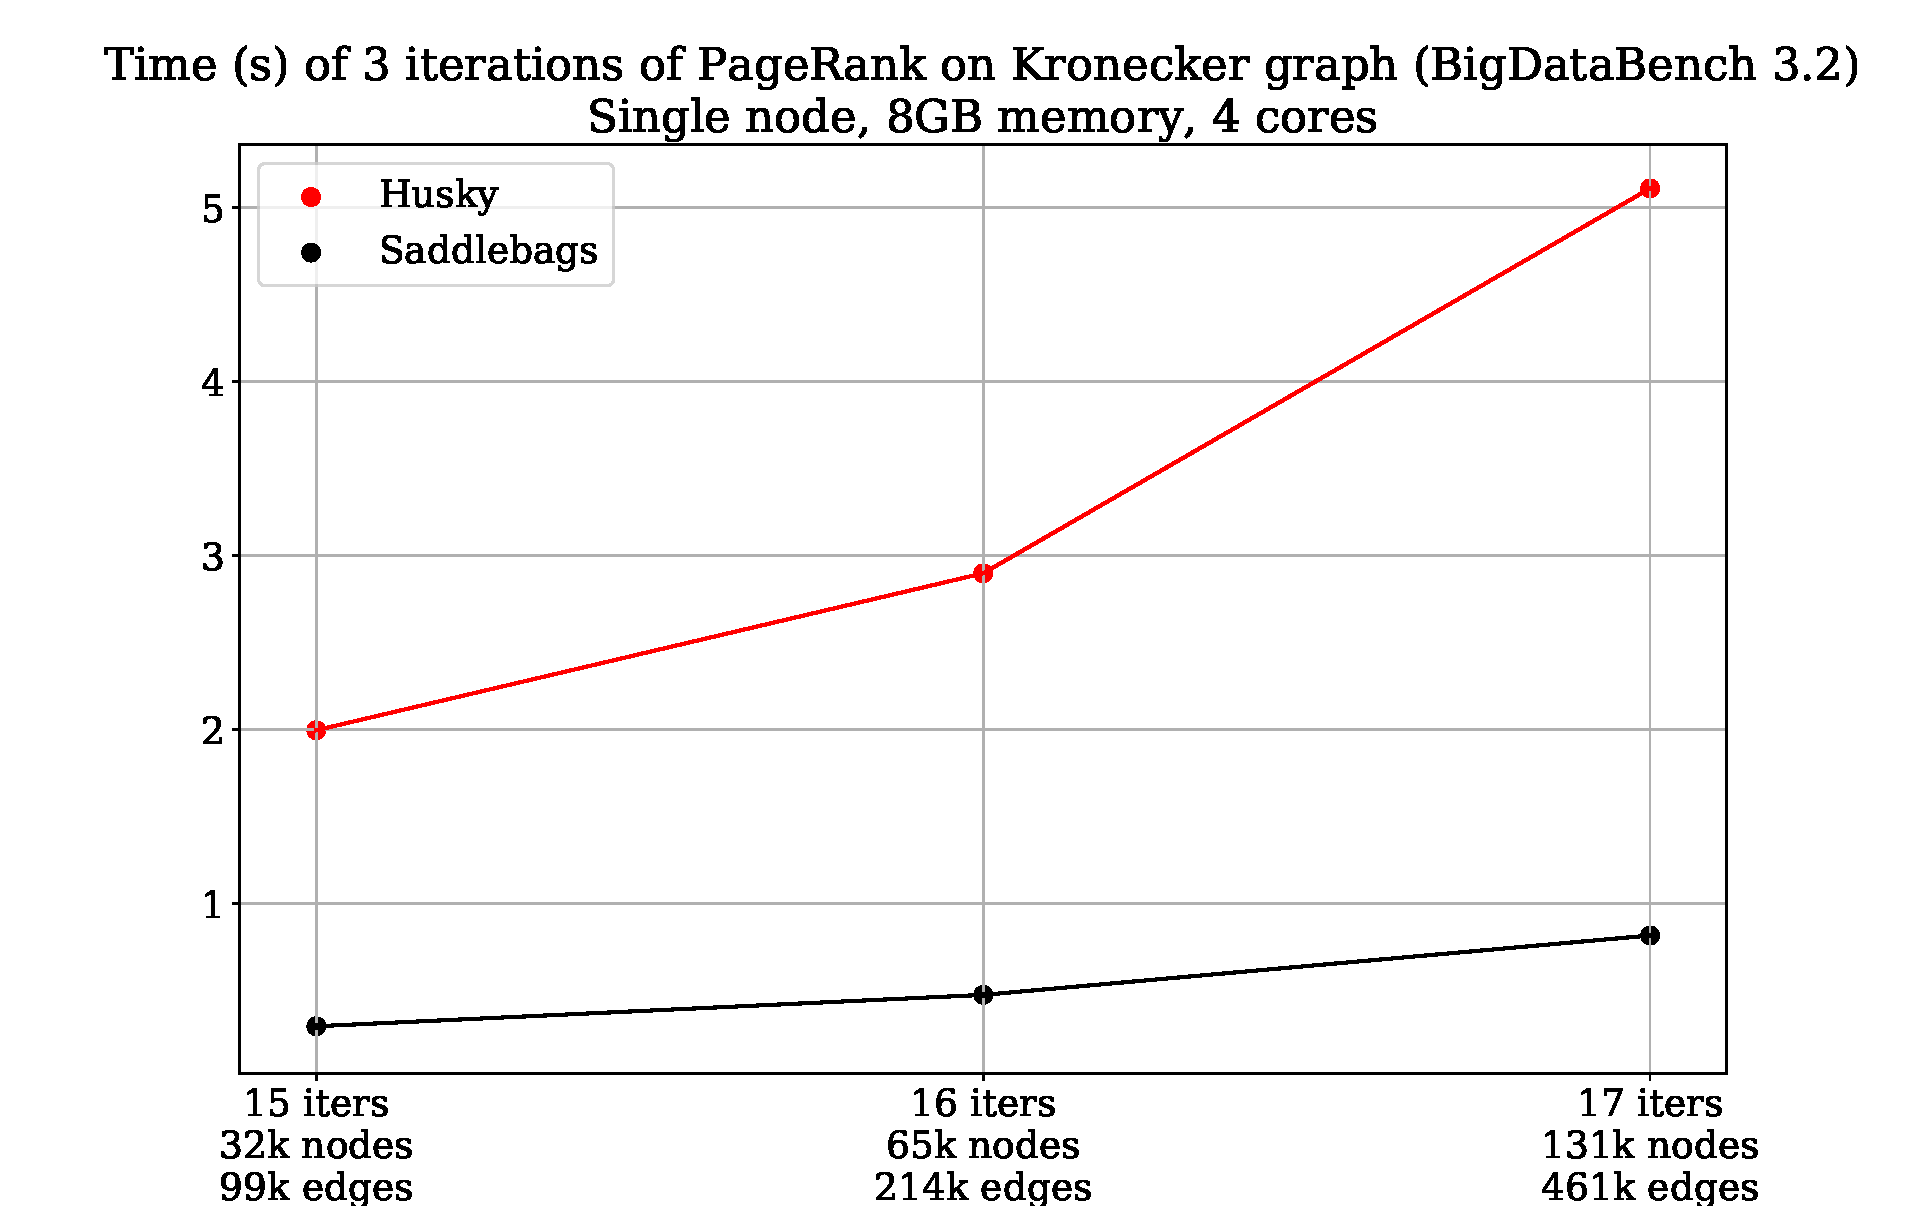
\includegraphics[width=8cm]{illustrations/huskypagerank.pdf}
	\caption{Execution time of PageRank in Saddlebags and Husky}
	\label{fig:huskypagerank}
\end{figure}


\subsection{Comparison with Spark}\label{section:sparkeval}
Comparisons with Spark were ran on the Abel cluster. For the PageRank benchmark, both a native Spark RDD MapReduce implementation, and a GraphX implementation, was used. GraphX is an API for running graph-based parallel jobs in Spark \cite{graphx}. Both the MapReduce \cite{sparkpagerank} and GraphX \cite{graphxpagerank} implementations were provided by official repositories. In thethe Spark implementation it is recommended to utilize GraphX to process this particular workload.

The other benchmark used with Spark is Term Frequency-Inverse Document Frequency (TF-IDF) \cite{tfidf}. This is an algorithm for classifying the relevance of words within a set of documents. A given word's importance within a given document is ranked based on its frequency within that document, and the inverse of the frequency of which it occurs in other documents. This benchmark was performed on a corpus of Wikipedia articles.

Results are shown in figure \ref{fig:sparkbench}. Both experiments show results that are significantly in favor of Saddlebags. These results are consistent with those presented in the Husky paper \cite{husky}, when using the comparison between Saddlebags and Husky from section \ref{section:huskycomp} as baseline. The advantage over Spark is explained by Husky as the result of fine-grained access of mutable data, which is also a relevant factor for Saddlebags, and applies to both benchmarks.

\begin{figure}[H]
	\centering
	\begin{subfigure}{8cm}
		\centering
		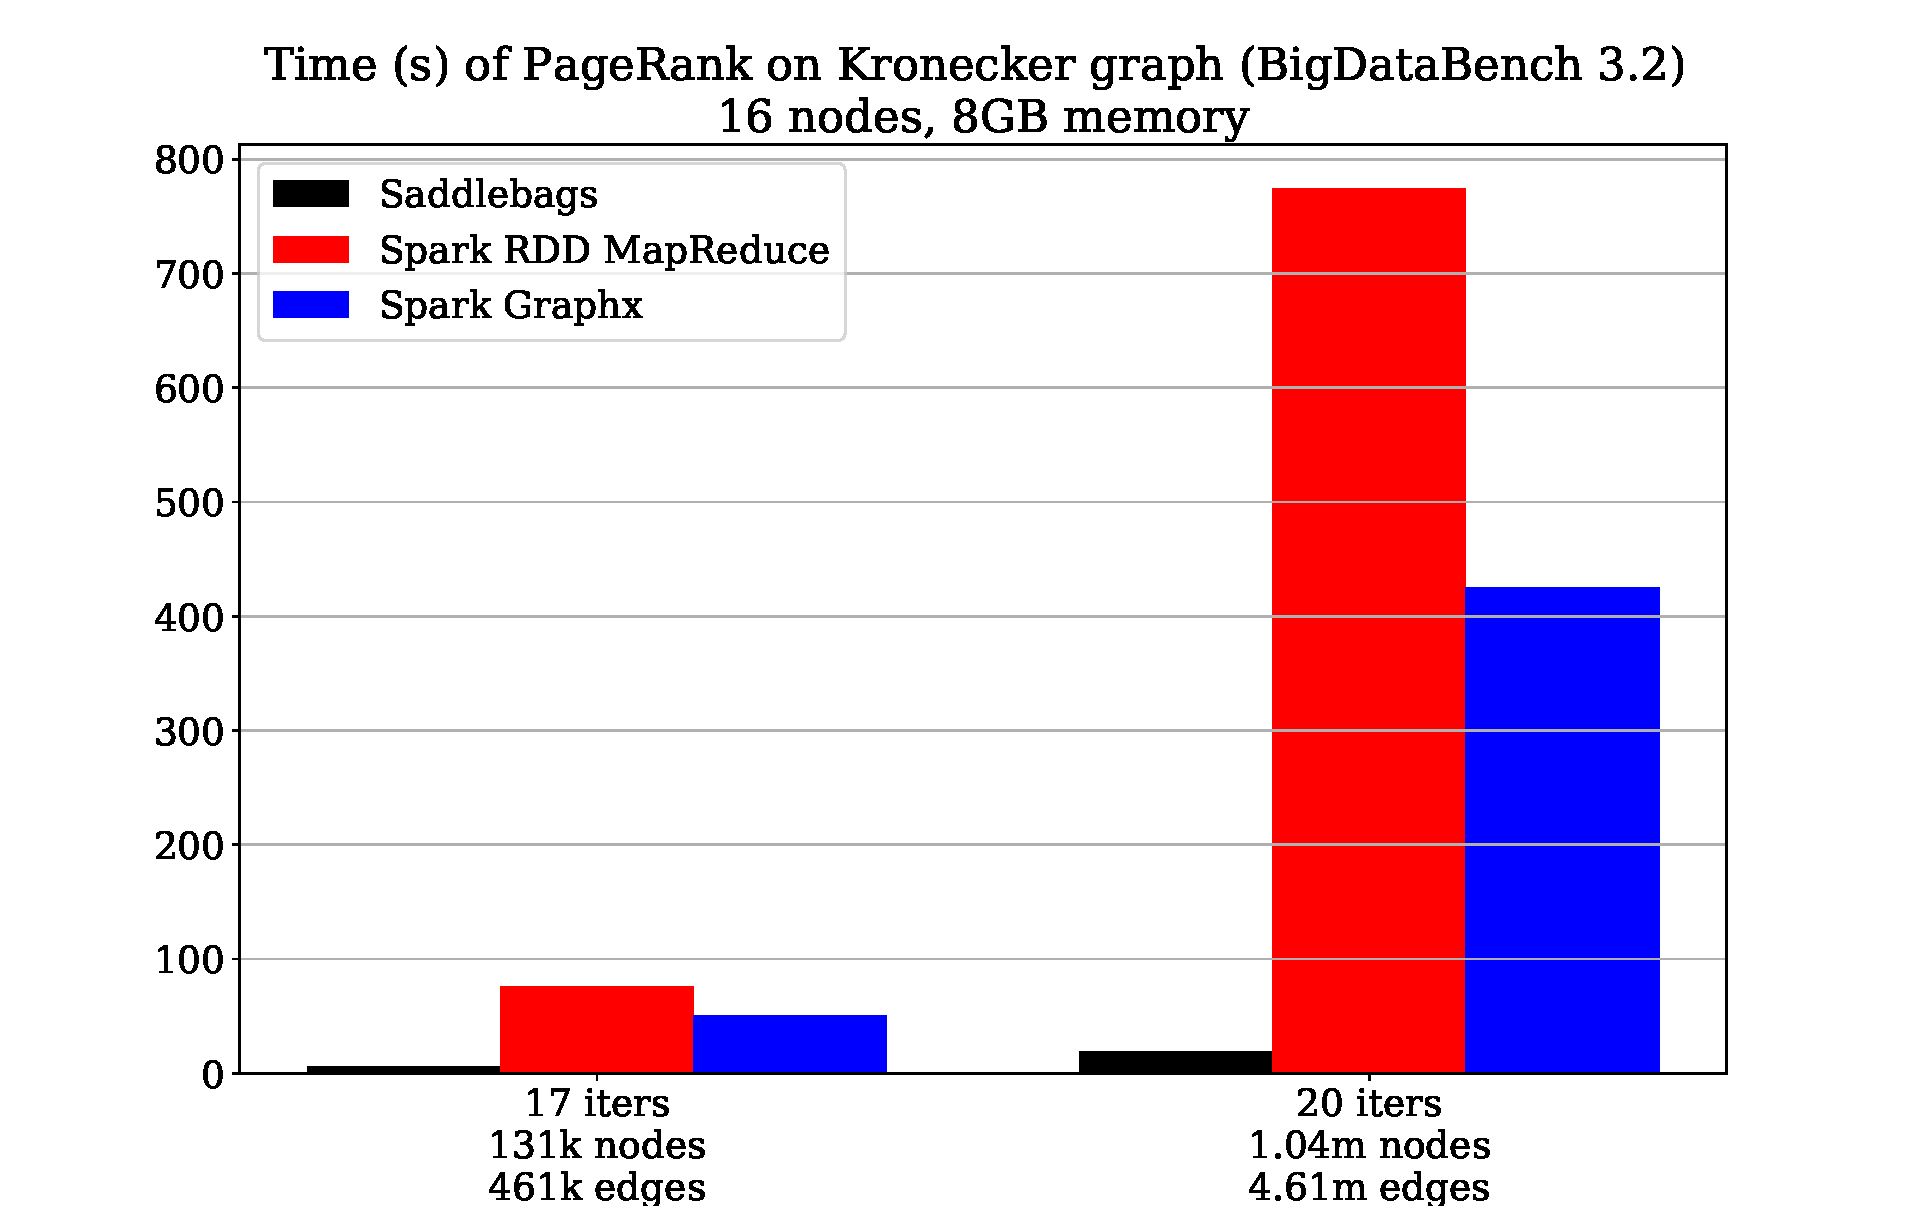
\includegraphics[width=8cm]{illustrations/sparkpagerank.pdf}
		\label{fig:sub1}
	\end{subfigure}%
	\begin{subfigure}{8cm}
		\centering
		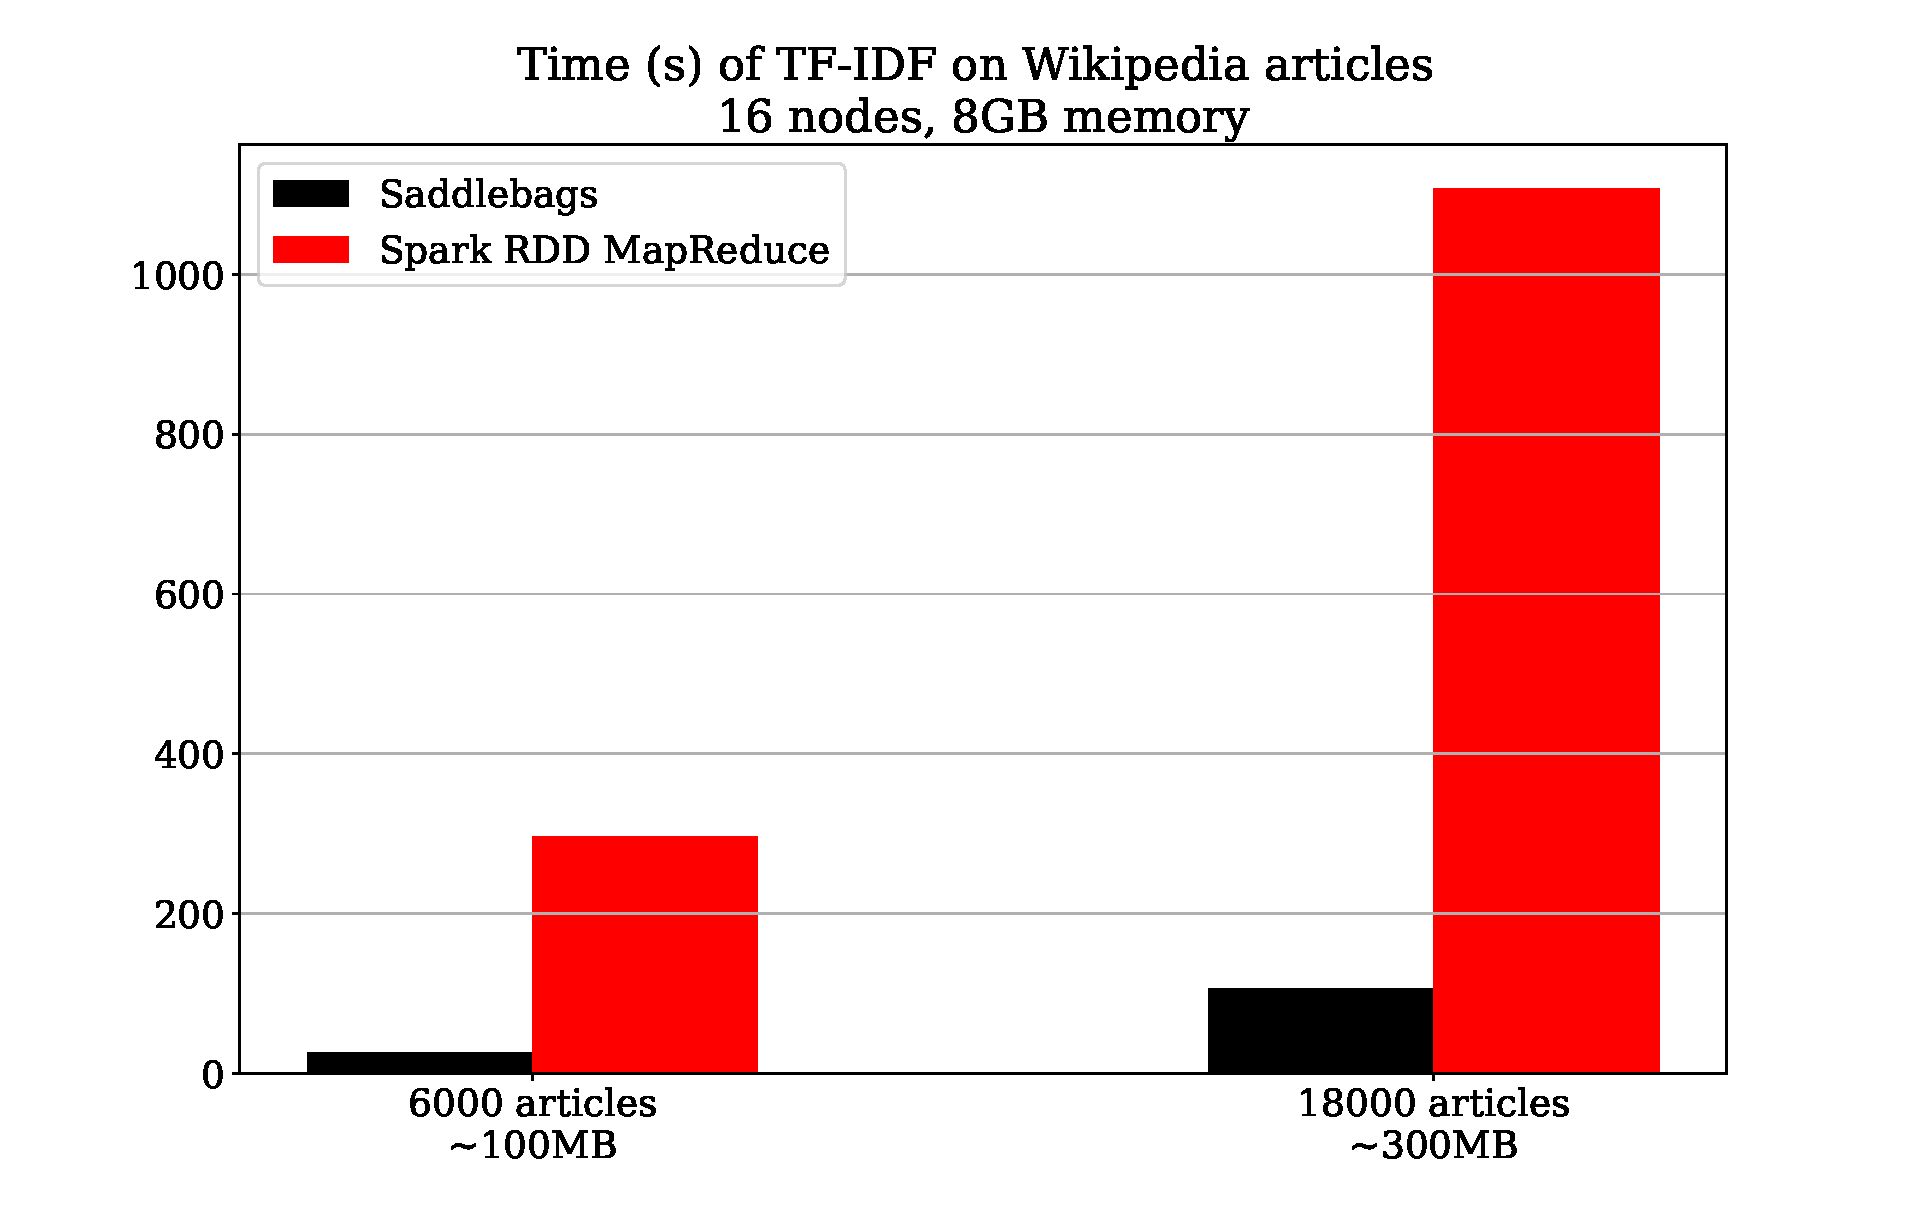
\includegraphics[width=8cm]{illustrations/sparktfidf.pdf}
		\label{fig:sub2}
	\end{subfigure}
	\caption{Execution time of PageRank and TF-IDF in Saddlebags and Spark}
	\label{fig:sparkbench}
\end{figure}


\subsection{Fault tolerance}\label{section:replicationeval}
The PageRank experiment from section \ref{section:huskycomp} was performed again with replication enabled, and the results are shown in figure \ref{fig:huskyfaulttolerance}.
The increase in execution time of the algorithm per degree of replication can be analyzed with linear regression. The relationship between average execution time and degree of replication on 17 iterations of the Kronecker graph can be mapped to the linear equation $Y = 0.1945X + 0.8445$ where $X$ is degree of replication and $Y$ is total execution time, with $r^2 = 0.984$, suggesting that this model is a good fit for the data. In practice, this means that adding a degree of replication in this experiment will increase the execution time with 0.1945 seconds, which is 23\% of the base execution time. While the time measurements are specific to this experiment, the significant observation is the linearity of the increase in time per replica. The implementation of the replication routine also implies that the increase in time should be linear, because the additional data movement required per additional replication node is constant.
\vskip 0.5cm
\begin{figure}[H]
	\centering
	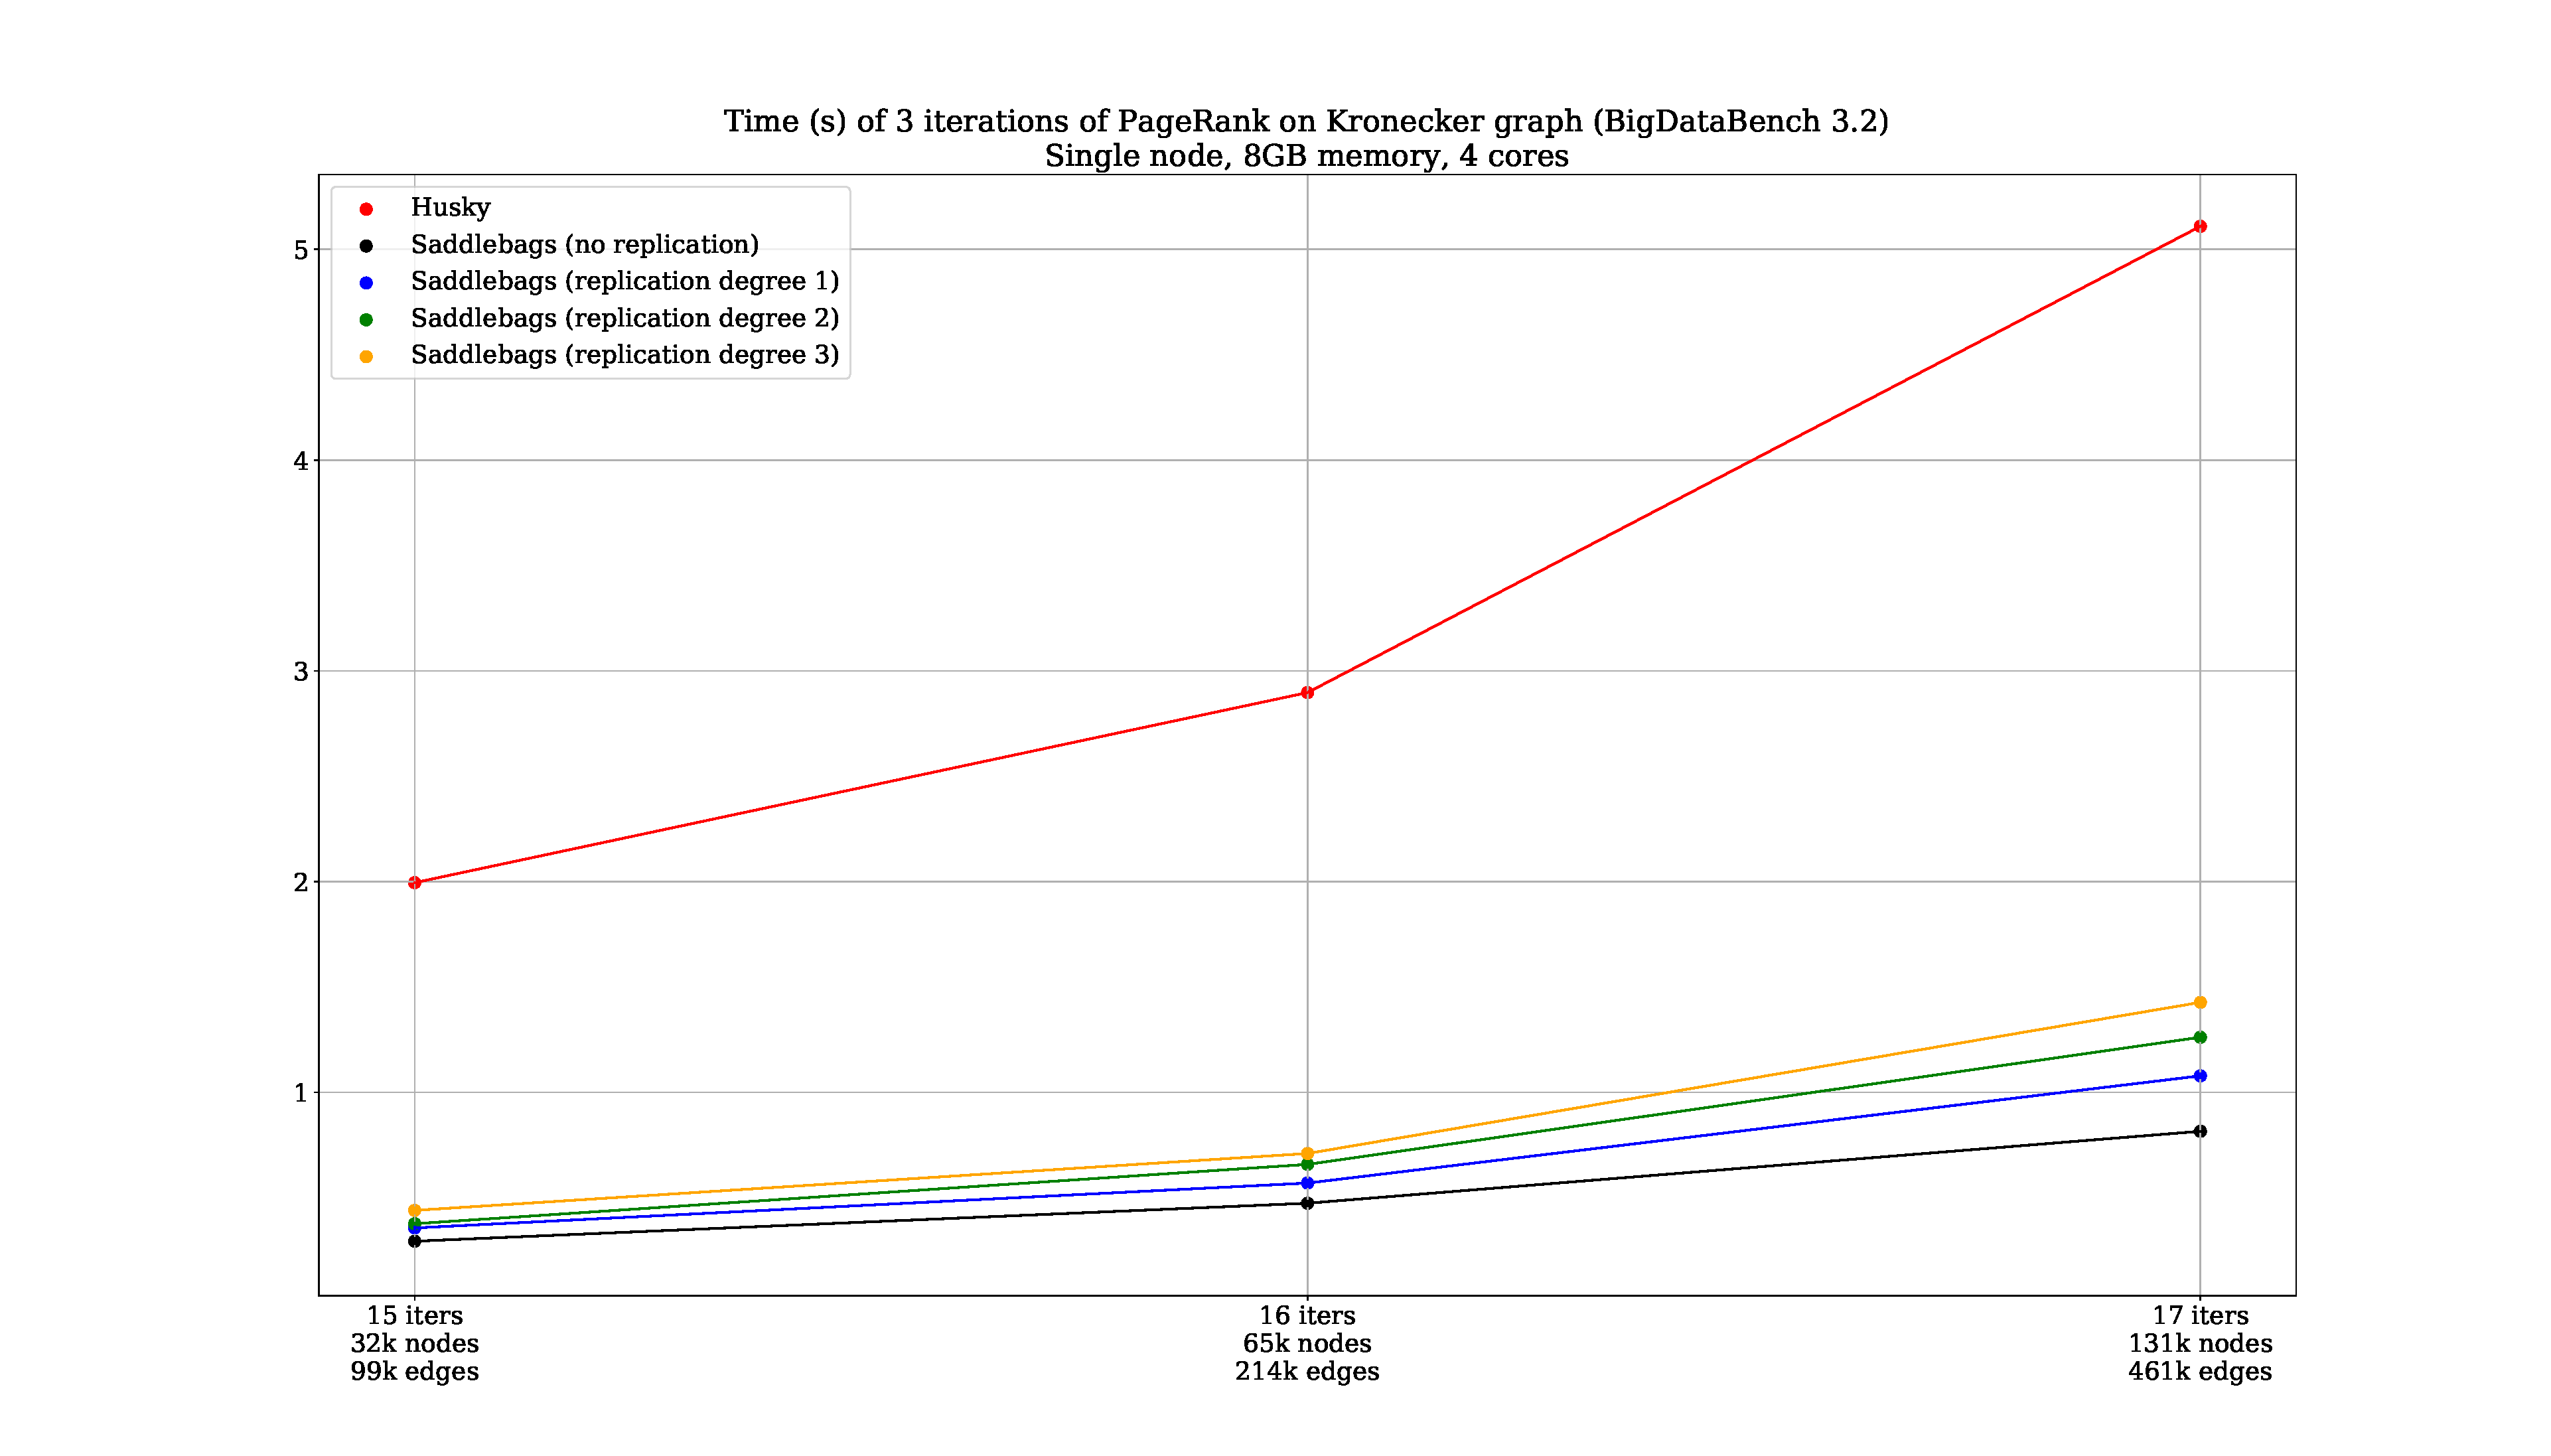
\includegraphics[width=11cm]{illustrations/replication.pdf}
	\caption{Execution time of PageRank in Saddlebags with replication}
	\label{fig:huskyfaulttolerance}
\end{figure}

\subsection{Sending modes} \label{section:sendingmodeseval}
Different sending modes were outlined in section \ref{section:sendingmodes}. The PageRank benchmark was ran with different sending modes to investigate their performance implications. This benchmark was performed on the 16 core server and the cluster with 16 nodes. Both systems were included because of how UPC++ and GASNet communication implementation differs from single nodes and distributed systems. On the server, communication is achieved through shared memory. On the cluster, communication is achieved through message passing over InfiniBand.

Figure \ref{fig:sendingmodes} shows results from this benchmark. In the single node environment, \\\texttt{GasnetBuffering} showed the worst performance. This sending mode avoids the Message abstraction, and achieves bulk synchronous parallel behavior by ignoring incoming RPCs until all local work has been completed. \texttt{Direct}, which also avoids the Message abstraction but handled RPCs immediately and disables bulk synchronous parallel behavior, showed the best performance, similar to \texttt{Buffering}. In the cluster environment, \texttt{Combining} showed the best performance by a significant margin, followed by \texttt{GasnetBuffering}. \texttt{Buffering} and \texttt{Direct} showed similar performance.

It is clear from these results that combining messages to reduce communication overhead is an effective technique in cluster environments. On single nodes, where communication is not executed through message passing, combining seems to have little effect, and may be unbeneficial because of the complexity introduced by the combination functionality.

\begin{figure}
	\centering
	\begin{subfigure}{8cm}
		\centering
		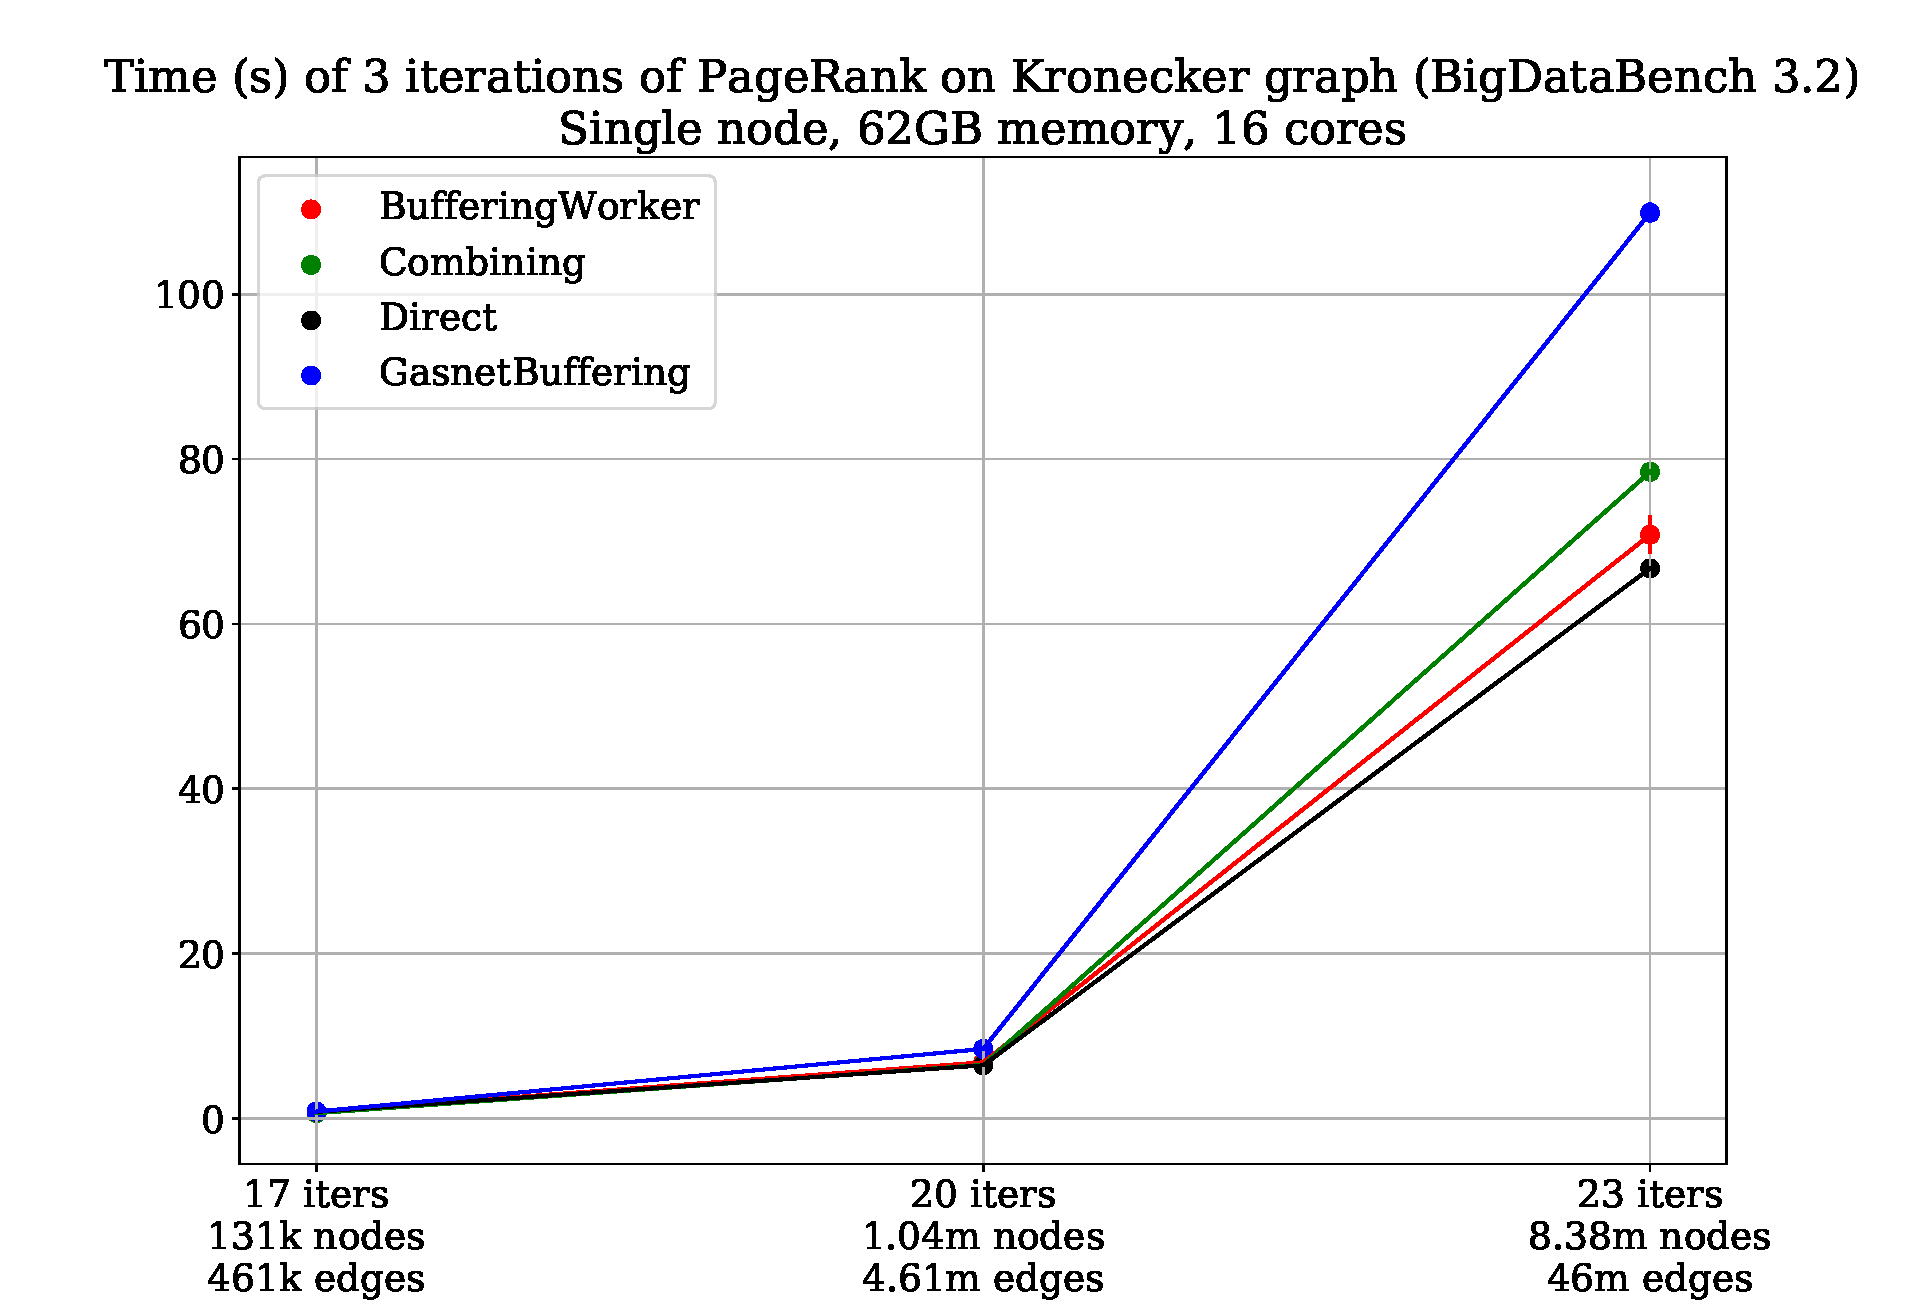
\includegraphics[width=8cm]{illustrations/sendingmodes.pdf}
		\label{fig:sub1}
	\end{subfigure}%
	\begin{subfigure}{8cm}
		\centering
		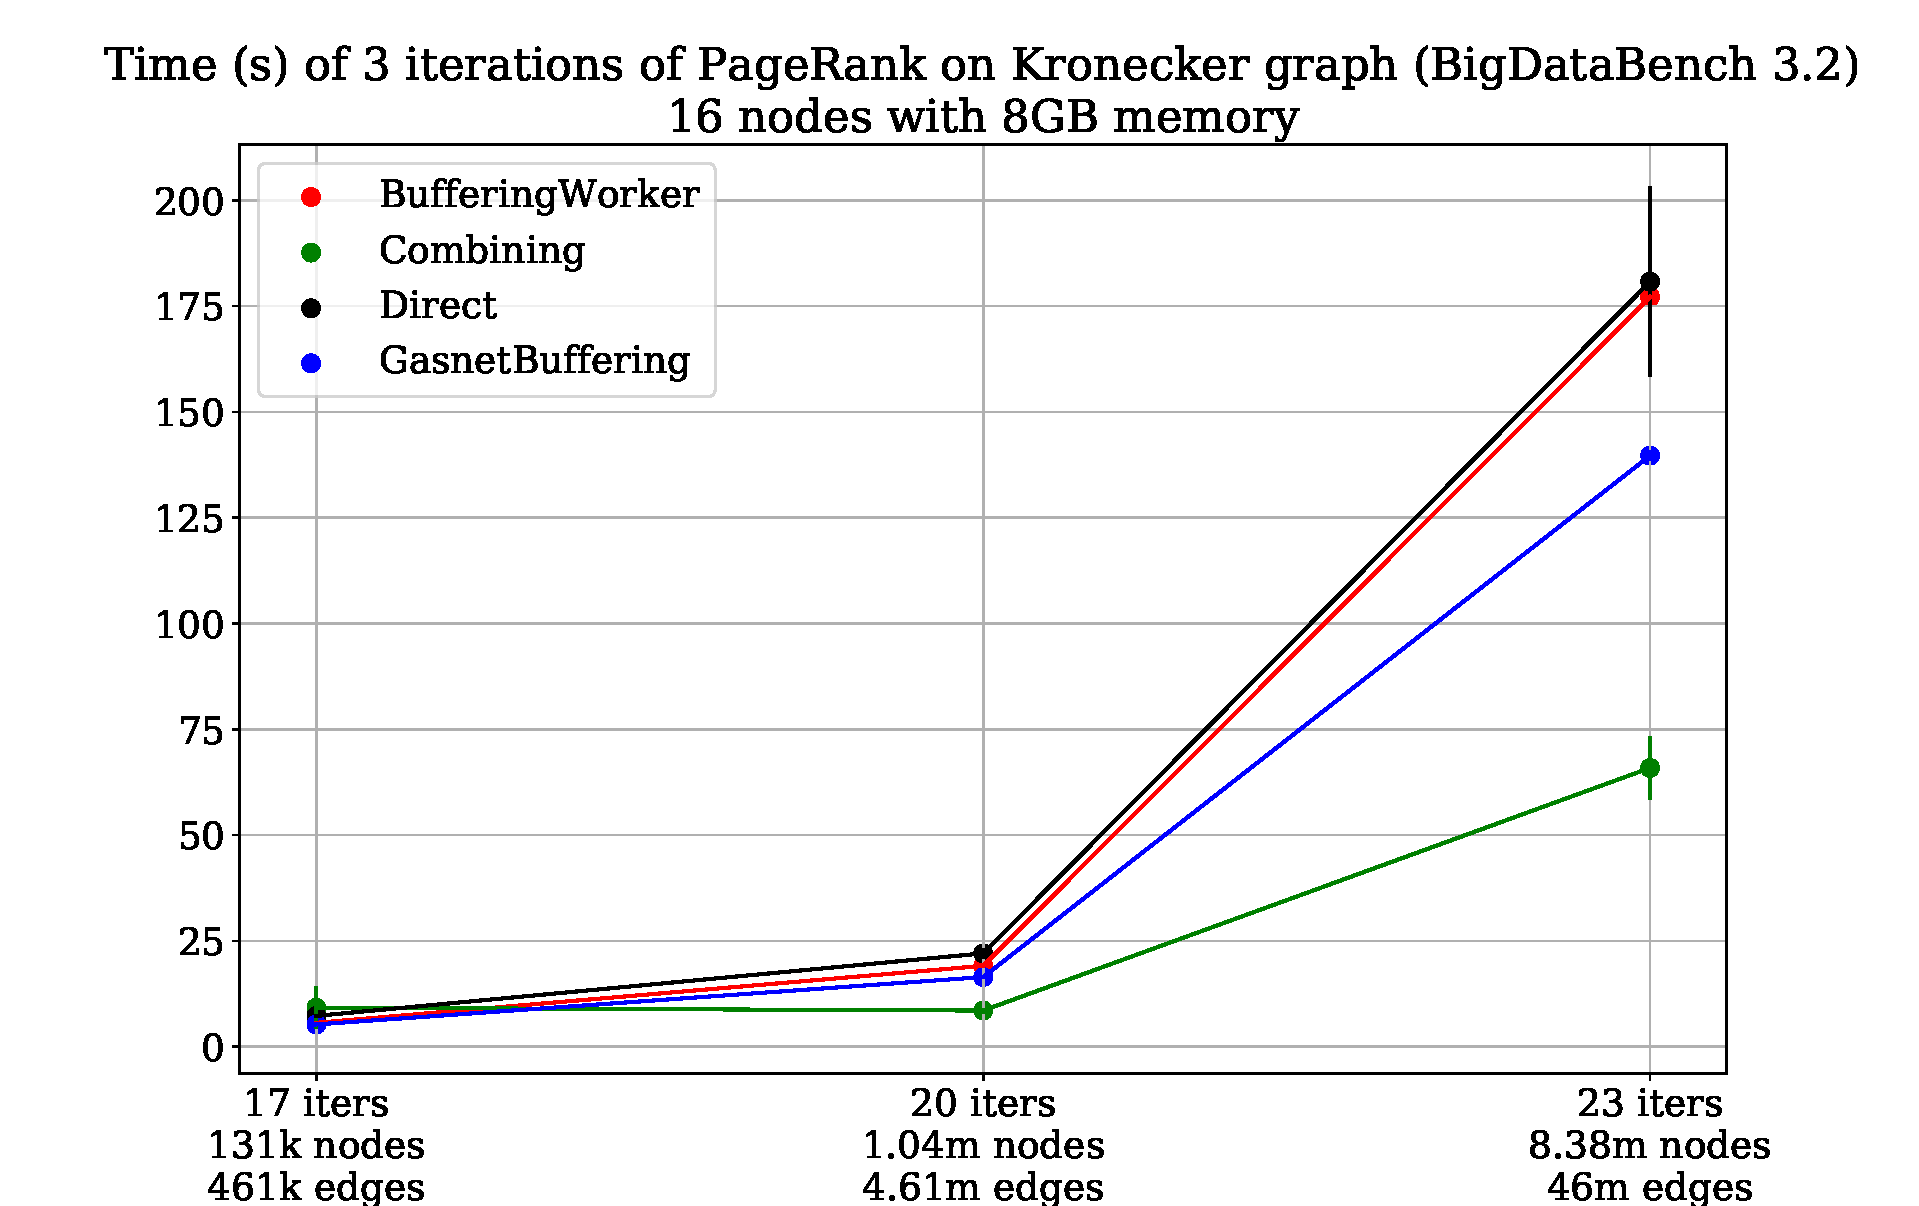
\includegraphics[width=8cm]{illustrations/sendingmodesabel.pdf}
		\label{fig:sub2}
	\end{subfigure}
	\caption{Execution time with different sending modes}
	\label{fig:sendingmodes}
\end{figure}


\section{Conclusion}
This thesis has presented Saddlebags, a High Performance Computing framework implemented in C++, using the UPC++ library for a partitioned global address space communication model. Saddlebags aims to provide support for workloads from the fields of both HPC and big data analysis. This is achieved by providing features from big data analysis that allows for easier programming and handling of large volumes of data, while providing a lightweight and customizable execution model. 

Saddlebags implements a bulk synchronous parallel programming model that is inspired by graph computing frameworks, but aims to support more diverse workloads. Saddlebags programs are based around extending a general-purpose data item class, that is accessible from all parallel partitions through RPCs. This base item class provides communication features and can be extended to execute computational tasks. Like UPC++, Saddlebags is customizable through C++ template programming.Fault tolerance is implemented with customizable in-memory replication techniques that has previously been used in various storage systems, in order to avoid the slowdown of accessing persistent storage. Several protocols for messaging between concurrent partitions have been implemented, with different performance characteristics and use-cases for programs running on individual machines and compute clusters.

Benchmarks shows that this approach, coupled with a communication layer implementation by UPC++ and GASNet, provides favorable performance in comparison with other contemporary systems for HPC and big data analysis. What is left for the future is a more extensive investigation of the various classifications of workloads that can benefit from the Saddlebags programming model.

\pagebreak
\bibliographystyle{ieeetr}
\bibliography{thesis}


% End of document
\end{document}
\grid
\grid




































